\documentclass{vldb}
\usepackage{graphicx}
\usepackage{caption}
\usepackage{float}


\begin{document}

% ****************** TITLE ****************************************

\title{Assignment 3 - DB2}

% ****************** AUTHORS **************************************

\numberofauthors{2} 

\author{
% 1st. author
\alignauthor Daniel Brand
% 2nd. author
\alignauthor Andreas Kostecka
}

\maketitle

\section{Relations and transactions}

\subsection{Implementing relations}

Points to discuss (not limited to):
\begin{itemize}
\item data structures chosen to store the relations
\begin{itemize}
\item \textbf{flights}
	\begin{verbatim}
		HashSet<Integer>
	\end{verbatim} 
	The \textit{HashSet} guarantees the uniqueness of flight IDs while providing a fast access due to hashing.
\item \textbf{seats} 
	\begin{verbatim}
		TreeMap<Integer, HashSet<Integer>>
	\end{verbatim}
	Since in this relation we have a mapping from a seat ID to a flight ID, the \textit{TreeMap} will be used, whose access times are fast. Furthermore, each seat ID can occur on many flights, whose ID is unique, so a seat ID will be mapped to a \textit{HashSet} of flight IDs.
\item \textbf{passengers}
	\begin{verbatim}
	HashSet<Integer>
	\end{verbatim}
	For the passengers a \textit{HashSet} will be used for the same reasons as for flights above.
\item \textbf{reservations}
	\begin{verbatim}
		TreeMap<Integer, 
		     HashSet<TreeMap<Integer, Integer>>>
	\end{verbatim}
	First of all a unique passenger may book a seat on several flights, so once again a \textit{TreeMap} is used for the mappings while a \textit{HashSet} stores the booked seats in flights. Another \textit{TreeMap} is used for the simple mapping of seat to flight ID. The reasons for this design decision is the same as stated above.
\end{itemize}
\item cardinality of the relations
\\In our simulated database there is a one-to-many relationship between passengers and reservations but only a one-to-one relationship between passengers and flights. So this means a passenger can have more than one reservation but only on different flights. It is not possible that a passenger can book multiple seats for one flight.
\\Furthermore we have a one-to-many relationship between one flight and seats.
\end{itemize}

\subsection{Implementing transactions}

Points to discuss (not limited to):
\begin{itemize}
\item \textbf{access methods of the transaction to the relations (read and write operations):}
\\In our design a transaction has no direct access to the database items. We implement already a simple class \textit{ConcurrencyControlManager.java} which provides access to our simulated database. For this assignment the class provides only simple access for getting and inserting data. In the further assignments we are going to implement also the complete locking in this class with the whole data structures needed. 
\\We provide the following read/write operations via the ConcurrencyManager:
\begin{itemize}
\item \textbf{getAllFlights}
	\begin{verbatim}
		Return: HashSet<Integer>
	\end{verbatim}
Returns all the unique flight IDs.
\item \textbf{getAllPassengers}
	\begin{verbatim}
		Return: HashSet<Integer>
	\end{verbatim}
Returns all the unique passenger IDs.
\item \textbf{getAllReservations}
	\begin{verbatim}
		Return: TreeMap<Integer, 
		     HashSet<TreeMap<Integer, Integer>>>
	\end{verbatim}
Returns all flights booked by all passengers.
\item \textbf{getSeatsPerFlightId}
	\begin{verbatim}
		Parameter values: Integer flightId
	\end{verbatim}
	\begin{verbatim}
		Return: HashSet<Integer>
	\end{verbatim}
Returns all seat IDs to the corresponding flight ID.
\item \textbf{deleteReservationByFlightAndPassengerId}
	\begin{verbatim}
		Parameter values: TreeMap<Integer, Integer> 
		reservation, Integer passengerId
	\end{verbatim}
Deletes a reservation from a passenger.
\item \textbf{insertReservationByPassengerId}
	\begin{verbatim}
		Parameter values: Integer passengerId,
		TreeMap<Integer, Integer> entry
	\end{verbatim}
	\begin{verbatim}
		Return: boolean
	\end{verbatim}
Inserts a reservation for a passenger.
\item \textbf{getReservationsByPassengerId}
	\begin{verbatim}
		Parameter values: Integer passengerId
	\end{verbatim}
	\begin{verbatim}
		Return: HashSet<TreeMap<Integer, Integer>>
	\end{verbatim}
Returns all flight reservations from a passenger.
\end{itemize}
Note: The operations may change in further assignments!
\item \textbf{properties of each transaction (operations to make, relations to access, interference with other transactions):}
\begin{itemize}
\item \textbf{book-Transaction}
\\This transaction books a reservation for a given seat on a flight. It invokes another transaction which checks first if the passenger has already booked a seat on the corresponding flight.
\item \textbf{cancel-Transaction}
\\This transaction cancels a reservation from a passenger. First this transaction calls another for checking if the reservation to delete exists. Then the transaction invokes another transaction for gaining all reservations from the passenger. Last the transaction calls the ConcurrencyControlMechanism-class to delete the reservation.
\item \textbf{myFlights-Transaction}
\\This transaction returns all the flight IDs where the passenger holds a reservation. Invokes a transaction from the ConcurrencyControlMechanism-class for getting all flights from a passenger.
\item \textbf{totalReservations-Transaction}
\\This transaction returns the sum of all reservations on all flights. It calls our implemented ''SUM''-function in the ConcurrencyControlMechanism-class.
\end{itemize}
Note: The properties may change in further assignments!
\item \textbf{distribution of the transactions which you consider for experimenting:} 
\\We want to do 2 variations of tests, one being deterministic and the other one will be randomized. The deterministic tests, i.e. tests whose results we know and can expect, will be used for immediate debugging while the randomized tests will do some pre defined amount of transactions with a random choice of transaction type (one of the 4 possible transactions). The deterministic ones will have a smaller amount of transactions whose types will also be pre defined, so we are talking about an uniform distribution for them.
\end{itemize}

\section{Serial schedules}
\subsection{Changelog}
Our previous implementation was messy and made scheduling hard. So we refactored our program in its entirety. A transaction is now an object with several properties. An agent creates a new \textit{DBTransaction} object and calls the now single public method \textit{exec} in \textit{ConcurrencyControlManager.java}. In the manager based on the transaction type the actual transactions will be done. By moving everything to here the locking should be become easier. The methods are still the same as documented in part 1.
\subsection{Points to discuss (not limited to)}
\begin{itemize}
\item \textbf{chosen mechanism to ensure serial schedules, especially in case of multiple threads:} \\All locking and scheduling happens in \textit{ConcurrencyControlManager.java}. To ensure a serial schedule, we created the 2 methods
\begin{itemize}
	\item private static synchronized void lockDatabase(int myId)
	\item private static void unlockDatabase(int myId)
\end{itemize}
which operate on the global lock \textit{databaseLock} of type \textit{Lock}. A description of \textit{Lock} is given in the next section. By adding the \textit{synchronized} keyword we ensure no second thread enters that method, so at any time only one thread even could lock the database. The function \textit{unlockDatabase} should not be synchronized, since no thread will ever move to that code until the first thread who locked the database unlocks it. Another mechanism is used in those aforementioned 2 methods. In every function a synchronized block surrounded by an infinite loop is located in the following form
\begin{verbatim}
while(true) {
  synchronized(databaseLock) {
    if(!databaseLock.open) continue;
    ...
    break;
  }
}
\end{verbatim}
The unlock method does not have the if - statement, so that this thread will actually unlock the database. By further synchronizing on the \textit{databaseLock} we avoid race conditions between the first and second thread, the first thread trying to unlock while the second tries to lock. The infinite loop has to be there to ensure that the second thread, i.e. the second transaction, stays the second thread. The two above methods are called (by wrapping in the two methods stated below) at the beginning and the end of a transaction respectively.
\item \textbf{implementation details of locking} \\For the locking part we introduced the 2 methods
\begin{itemize}
	\item lockManagementGrowing(DBTransaction transaction)
	\item lockManagementShrinking(DBTransaction transaction)
\end{itemize}
and the static subclass \textit{Lock} of our manager. The subclass \textit{Lock} has the following fields
\begin{itemize}
	\item LockType type (either LOCK-S or LOCK-X)
	\item boolean open (open == true means open lock)
	\item HashSet$<$Integer$>$ agentIDs (will be important later on)
\end{itemize}
The type of a lock was not important for this part but will surely be later on for 2PL. The \textit{open} field is the important part. The usage of agentIDs is already simulated in database locking but was not essential. A global variable called \textit{serial} defines which scheduling scheme will be used.
\end{itemize}

\section{2PL and concurrency}
\subsection{Changelog}
\begin{itemize}
\item \textbf{Data-Structures}\\
We simplified the data-structure of our reservations from
	\begin{verbatim}
		TreeMap<Integer, 
		     HashSet<TreeMap<Integer, Integer>>>
	\end{verbatim}
to
	\begin{verbatim}
		TreeMap<Integer, TreeMap<Integer, Integer>>
		TreeMap<PASSENGER-ID, 
		     TreeMap<FLIGHT-ID, SEAT-ID>>
	\end{verbatim}
\item \textbf{Choosing a free seat}\\
We return now the list of all possible free seats of a flight to the passenger. The passenger chooses then randomly a free seat from the list for booking.
\item \textbf{Test-Cases}\\
Our test-cases are now more realistic. The transaction occurrences have the following order \textit{book \textgreater cancel \textgreater myFlights \textgreater totalReservations}. Furthermore we split the manager class into 3 sub classes. In the class \textit{ConcurrencyControlManager} we kept all about locking and scheduling, the class \textit{DBAccess} has all direct database access methods with a corresponding SQL statement as a comment above them to indicate, what we actually do in those methods. The third class is called \textit{DBConnection} and is now our interface to the outside, i.e. the method \textbf{exec} is now in there, together with the transactions and calls to DBAccess and ConcurrencyControlManager.
\end{itemize}
\subsection{Points to discuss (not limited to)}
\begin{itemize}
\item \textbf{types of implemented locks} The locks we implemented are \textbf{LOCK-S} and \textbf{LOCK-X}. We thought we had to strictly keep to the lecture notes for \textit{Datenbanken Vertiefung} where those two are the only discussed lock types for the \textbf{2PL} chapter. In our current implementation sometimes the concurrent modification exception is thrown, because for the following possible and not so unprobable schedule:
\begin{itemize}
	\item Transaction X acquires an exclusive lock on data A. Before acquisition any conflicting lock was accounted for, i.e. a transaction waits until every conflicting lock gets released
	\item While X waits, another transaction Y acquires some other lock on either data A or on the whole table and starts its works. Transaction X however never re-checks for conflicting locks.
	\item Now transaction X can finally start and starts removing tuples or does any kind of write(A).
	\item Since Y wants to read that data A and has acquired a shared lock on data A, this transaction runs into an exception.
\end{itemize}
So we have an existing problem with exclusive locks which can be easily solved by using an intentional exclusive lock on the table. We will fix this problem until the next assignment. As briefly discussed above, we support table and row or tuple locks.
\item \textbf{implementation details of the concurrency mechanism (requesting/granting locks)} The locking magic happens in the class \textit{ConcurrentControlManager} within the two methods \textbf{lockManagementGrowing} and \textbf{lockManagementShrinking}. The names should imply which method does what. In our implementation the shrinking phase happens exactly at the end of each transaction, so the growing phase lasts right until the end of a transaction. As requested for the \textbf{2PL} scheme no lock gets released/removed until the shrinking phase begins and whilst shrinking no lock can be acquired. The following variables are essential for our locking mechanism:
\begin{itemize}
	\item HashSet$<$Lock$>$ flightLocks
	\item HashSet$<$Lock$>$ seatLocks
	\item HashSet$<$Lock$>$ passengersLocks
	\item HashSet$<$Lock$>$ reservationLocks
	\item TreeMap$<$Integer, HashSet$<$Lock$>>$ locksPerTransaction
	\item Lock flightsTableLock
	\item Lock seatsTableLock
	\item static Lock passengersTableLock
	\item static Lock reservationsTableLock
\end{itemize}
The sets of locks are used for row/tuple locking for their respective table as indicated by the names of the sets. The locks of type \textbf{Lock} are used as table locks. The data structure of \textit{Lock} is discussed below. The variable \textit{locksPerTransaction} is essential for our shrinking phase. In the method \textit{lockManagementShrinking} a transaction simply opens and/or removes any lock held by that transaction. Those lock references are kept in a \textit{HashSet} and are mapped to the unique \textit{agentId} of a thread. Since any thread can only do one transaction at a time, this mapping is unique in turn. Further information is saved in the \textbf{Lock} data structure with the following fields:
\begin{itemize}
	\item LockType type;
	\item LockStatus status;
	\item HashSet$<$Integer$>$ agentIDs;
	\item DBStructure.Table table;
	\item Integer row;
	\item Integer flightId;
\end{itemize}
As discussed above the lock type can either be \textbf{LOCK-S}, \textbf{LOCK-X} or for convenience while debugging \textbf{UNSET}. The status of a lock is now an \textit{enum}. A lock can have status \textbf{OPEN}, \textbf{LOCKED} or \textbf{REMOVED}. The status \textit{REMOVED} is only used for tuple locking while a table lock is either \textit{OPEN} or \textit{LOCKED}. The \textit{agentIDs} are for table locks. Tuple locks are created for each transaction, i.e. multiple \textit{LOCK-S} locks on one row exist multiple times. The last 3 fields of the data structure \textit{Lock} are important for the shrinking and growing phase alike. So we save for which table that lock was granted and on which data. The field \textit{flightId} is or can be used for the tables \textit{seats} and \textit{reservations}.
\paragraph*{growing phase} This phase is built up as follows:
\begin{enumerate}
	\item Check for a conflicting table lock and remember it
	\item Check for conflicting row/tuple locks and remember them
	\item Wait for each remembered lock until status either becomes \textit{OPEN} or \textit{REMOVED}
	\item Always check for timeout, in case of timeout, abort transaction
	\item If no timeout occurred any conflict could be solved so either create a new lock (tuple locking) or set a table lock to \textit{LOCKED}
\end{enumerate}
The method \textit{lockManagementGrowing} is called in DBConnection right before a call to a function in DBAccess. At the end of the growth function either a lock reference or null is returned. If DBConnection receives a null pointer the transaction aborts.
\end{itemize}

\section{Experiments}
\subsection{Changelog}
Once again we had to rearrange or modificate a few things here and there. Notable this time is the implementation of \textit{multiple granularity locking}. So now we have the lock types IS, S, IX and X. The lock type SIX is defined but unused. As per definition in the lecture notes we first lock our table either in IS or IX and then the wanted tuple, in case of reading or writing a whole table S and X are set on the table. Furthermore we now support granularity escalations. Should a compatible lock be granted on an already locked table that older luck gets a higher granularity. The new method
\begin{verbatim}
ConcurrencyControlManager.
 isCompatible(LockType type1, LockType type2)
\end{verbatim}
represents the multiple granularity locking matrix by comparing two given lock types. Another new method is called
\begin{verbatim}
ConcurrencyControlManager.
 determineWantedTableLockType(
   LockType wantedType, boolean tableLock)
\end{verbatim}
where we map a wanted lock to a table lock type. A thread may request only LOCK-S or LOCK-X on a tuple but the table then requires an intentional lock. The returned type of this method is then compared to an existing lock on a table by using above function.
\subsection{Points to discuss (not limited to)}
\begin{itemize}
\item \textbf{experiments setup (programming language, transaction distributions, measures)} Our implementation is written in Java. For multithreading we created a subclass of \textit{Thread}, those threads are then started with \textit{.start()} and by calling \textit{.join()} in the main process on those threads we wait for their termination.
\item \textbf{each experiment (method, results, findings)} We got one interesting result. Our implementation of serial and 2PL seem to scale at the same pace with a growing agent or thread count as seen in \ref{impact}. No matter how much time we invested to find an error within our implementation we could not locate any. This leads to our guess that maybe Java, OS or the hardware do something behind the scenes. For each test run with a different amount of threads we recreated the data structures, but did that in the same way. So maybe something gets cached and thus becomes real fast while accessing. We could not determine the real cause though. The expected result for serial would have been for the throughput to stay constant independent to the thread count, since in serial mode at any time only a single process can execute the query.
\begin{figure}[H]
	\centering
	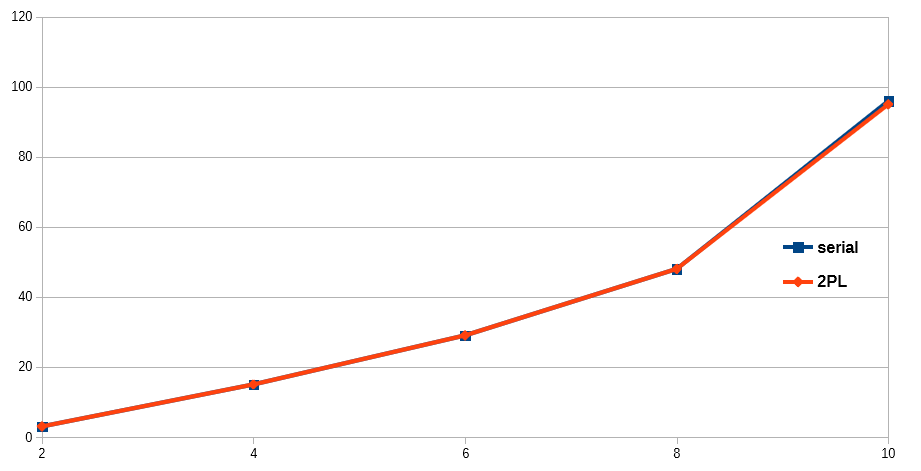
\includegraphics[width=.46\textwidth]{impact.png}
	\caption{Throughput in 1/s with varying agent count}
	\label{impact}
\end{figure}
\end{itemize}

\end{document}